% =========================================================================== %
% Yes. This is a document.

\documentclass[
	english,
	aspectratio=169,
	table
]{beamer}

% =========================================================================== %
% Theme
\usepackage{scrlfile}
	\ReplacePackage{beamerthemeSHUR}{./sty/beamerthemeSHUR}
	\ReplacePackage{beamerinnerthemefancy}{./sty/beamerinnerthemefancy}
	\ReplacePackage{beamerouterthemedecolines}{./sty/beamerouterthemedecolines}
	\ReplacePackage{beamercolorthemechameleon}{./sty/beamercolorthemechameleon}

\usetheme[
	pageofpages=/,
	bullet=circle,
	titleline=true,
	alternativetitlepage=true,
	watermark="",
	watermarkheight=0px,
	watermarkheightmult=0
	]
{SHUR}

% =========================================================================== %
% the usual stuff

\usepackage[utf8]{inputenc}
\usepackage[T1]{fontenc}
\usepackage{babel}
\usepackage{lmodern}
\usepackage{microtype}
\usepackage{csquotes}

\usepackage{tabularx}
\usepackage{booktabs}
\usepackage{multirow}

\usepackage{color, colortbl}
\usepackage{xcolor}
	\definecolor{tabhighlight}{RGB}{230,240,255}
	\definecolor{tabcontrast} {RGB}{200,210,255}

\usepackage{tabto}
\usepackage{xspace}

% math
\usepackage{amsmath}
\usepackage{amssymb}
\usepackage{dsfont}
\usepackage[arrowdel]{physics}
\usepackage{mathtools}
\usepackage{siunitx}

\usepackage{minted}
	\usemintedstyle{friendly}

\usepackage{tikz}
	\usetikzlibrary{positioning}
	\usetikzlibrary{matrix}
	\usetikzlibrary{shapes.geometric}
	\usetikzlibrary{backgrounds}
	\usetikzlibrary{calc}
	\usetikzlibrary{decorations.pathreplacing}
	\usetikzlibrary{arrows}
\usepackage{adjustbox}

\usepackage[most]{tcolorbox}
	\tcbsetforeverylayer
		{colback=cyan!10!white,
		 colframe=cyan!75!black,
		 arc=0pt,
		 outer arc=0pt,
		 parbox=false
		}
	\newtcolorbox{codebox}[1][Code]
		{colback=black!5!white,
		 colframe=blue!40!black,
		 title=#1,
		 leftupper=6mm
		}
	\newtcolorbox{cmdbox}[1][Kommandozeilen-Befehl]
		{colback=black,
		 coltext=white,
		 fontupper=\ttfamily ,
		 colframe=blue!40!black,
		 title=#1,
		 outer arc=0pt
		}
	\newtcolorbox{warnbox}[1][Beachte]
		{colback=black!5!white,
		 colframe=red!40!black,
		 title=#1
		}
	\newtcolorbox{hintbox}[1][Tipp]
		{colback=black!5!white,
		 colframe=green!40!black,
		 title=#1
		}
	\newenvironment{itembox}
		{\begin{tcolorbox}\begin{itemize}}%
		{\end{itemize}\end{tcolorbox}}
	\newtcolorbox{doublebox}[1][.3]
		{righthand width=#1\linewidth,
		 sidebyside,
		 sidebyside gap=6mm,
		 sidebyside align=center,
		 lower separated=false}
	
%==============================================================================%
% GLOBAL MACROS

\newcommand*{\eg}{e.\,g. }
\newcommand*{\ie}{i.\,e. }

\newcommand{\Thus}{\ensuremath{\Rightarrow}\xspace}
\newcommand{\thus}{\ensuremath{\rightarrow}\xspace}

\newcommand*{\tabcrlf}{\\ \midrule}			% actually still allows for optional argument

\newcommand*{\inPy}[1]{\mintinline{python3}{#1}}

% =========================================================================== %

\author{Stefan Hartinger}
\title{Programming in Python}
\subtitle{Part 15+16: The MatPlotLib}
\institute{University Regensburg, Department of Theoretical Physics}
\date{Block Course, Summer Term 2021}

% =========================================================================== %

\begin{document}
% =========================================================================== %

\begin{frame}[t,plain]
\titlepage
\end{frame}

% =========================================================================== %

%\begin{frame}{Recap}
%%
%\begin{columns}[T]
%\column{.5\linewidth}
%\begin{itemize}
%\item Exceptions
%\item Block structure
%	\begin{itemize}
%	\item \inPy{try}: Anything that might go wroing
%	\item \inPy{except}: What to do if something goes wrong
%	\item \inPy{else}: What to do if everything is all right
%	\item \inPy{finally}: What to do in any case
%	\end{itemize}
%\item Error Classes
%	\begin{itemize}
%	\item Hierarchical Order
%	\item Allows specific treatment
%	\end{itemize}
%\end{itemize}
%%
%\column{.5\linewidth}
%\begin{itemize}
%\item Command \inPy{raise}
%	\begin{itemize}
%	\item Trigger an exception yourself
%	\item Argument: instance of an error class
%	\item Or: Re-raise in an \inPy{except} block
%	\end{itemize}
%\item Own Error Classes
%	\begin{itemize}
%	\item Inherit from \texttt{Exception}
%	\item Arbitrary Design
%	\item Usually only for specific treatment of user-defined errors: \enquote{empty} classes
%	\end{itemize}
%\end{itemize}
%
%\end{columns}
%%
%\begin{center}
%	\emph{Any Questions?}
%\end{center}
%%
%\end{frame}

% =========================================================================== %

%\begin{frame}{Recap}
%%
%\begin{columns}[T]
%\column{.5\linewidth}
%\begin{itemize}
%\item Manipulating the file cursor
%	\begin{itemize}
%	\item \texttt{handle.tell} -- get current position
%	\item \texttt{handle.seek(offset, startPoint)} -- move file cursor
%	\end{itemize}
%\item Pickle
%	\begin{itemize}
%	\item Serialize objects
%	\item Works with (virtually) everything in Python
%	\item May contain (harmful) code
%	\item \texttt{pickle.dump} and \texttt{pickle.load}
%	\end{itemize}
%\end{itemize}
%%
%\column{.5\linewidth}
%\begin{itemize}
%\item JSON
%	\begin{itemize}
%	\item Inter-Plattform serialization
%	\item Only works with specific data types
%	\item Human readable format
%	\item \texttt{json.dump} and \texttt{json.load}
%	\item Usually: \inPy{dict}s of variables
%	\end{itemize}
%\item CSV
%	\begin{itemize}
%	\item Data in columns
%	\item Class \texttt{DictReader} via \texttt{csv.reader}
%	\item Iterable -- can be used with \inPy{for}
%	\item Rows split into columns by a separator character (\eg \texttt{','}) into \inPy{list}s
%	\end{itemize}
%\end{itemize}
%
%\end{columns}
%%
%\begin{center}
%	\emph{Any Questions?}
%\end{center}
%%
%\end{frame}

% =========================================================================== %

%\begin{frame}[fragile]
%%
%\begin{tcbraster}[raster columns=2,
%                  raster equal height,
%                  nobeforeafter,
%                  raster column skip=0.5cm]
%\begin{codebox}[Example: Title goes here]
%\begin{minted}[fontsize=\scriptsize, linenos]{python}
%foo
%\end{minted}
%\end{codebox}
%%
%\begin{codebox}[Example: Title goes here]
%\begin{minted}[fontsize=\scriptsize, linenos]{python}
%bar
%\end{minted}
%\end{codebox}
%\end{tcbraster}
%%
%\end{frame}

% =========================================================================== %

\begin{frame}[fragile]{Chapter 10}
%
\begin{itemize}
\item Basics of the MatPlotLib
\item Manipulating Plot Details
\item Different Plot Types
\item Object Oriented Approach
\item 3D Plots
\item Saving Plots into Files
\end{itemize}
%
\end{frame}

% =========================================================================== %

\begin{frame}[fragile]{A First Example}
%
\begin{codebox}[Example: A Simple Plot, width=.53\linewidth, nobeforeafter, equal height group = grpXmpSimplePlot]
\begin{minted}[linenos, fontsize=\scriptsize]{python3}
import math
import matplotlib.pyplot as plt

N = 100
X = [(x - N/2) / 10 for x in range(N)]
Y = [math.sin(x) for x in X]

plt.plot(X, Y)
plt.show()
\end{minted}
\end{codebox}
%
\begin{tcolorbox}[title=Output: A Simple Plot, width=.45\linewidth, nobeforeafter, equal height group = grpXmpSimplePlot]
	\includegraphics[width=\linewidth]{./gfx/plt-sin}
\end{tcolorbox}
%
\end{frame}

% =========================================================================== %

\begin{frame}[fragile]{Code Analysis}
%
\begin{itemize}
\item \inPy{import matplotlib.pyplot as plt}
	\begin{itemize}
	\item Module \texttt{matplotlib.pyplot} brings tons of functions
	\item Highly complex structure -- organized into sub-modules
	\item Convention: load as \texttt{plt} to spare us typing this over and over
	\end{itemize}
\item Objects \texttt{X, Y}
	\begin{itemize}
	\item Data to plot
	\item Simple lists of numbers
	\item Same length
	\item Coordinates
	\end{itemize}
\item \inPy{plt.plot(X, Y)}
	\begin{itemize}
	\item Prepare the plot in memory
	\item Allows for alterations to the default settings
	\end{itemize}
\item \inPy{plt.show()}
	\begin{itemize}
	\item \enquote{Go live}
	\item Show the plot on screen
	\item Wait with execution until plot window is closed
	\end{itemize}
\end{itemize}
%
\end{frame}

% =========================================================================== %

\begin{frame}[fragile]{Adding Some Details}
%
\begin{codebox}[Example: Plot with Grid and Legend, width=.49\linewidth, nobeforeafter, equal height group = grpXmpGrid]
\begin{minted}[linenos, fontsize=\scriptsize]{python3}
import math
import matplotlib.pyplot as plt

N  = 100
X  = [(x - N/2) / 10 for x in range(N)]
Y1 = [math.sin(x) for x in X]
Y2 = [math.cos(x) for x in X]

plt.plot(X, Y1, label="Sinus")
plt.plot(X, Y2, label="Cosinus")

plt.legend()
plt.grid()

plt.show()
\end{minted}
\end{codebox}
%
\begin{tcolorbox}[title=Output: Plot with Grid and Legend, width=.49\linewidth, nobeforeafter, equal height group = grpXmpGrid]
	\includegraphics[width=\linewidth]{./gfx/plt-grid}
\end{tcolorbox}
%
\end{frame}

% =========================================================================== %

\begin{frame}[fragile]{Code Analysis}
%
\begin{itemize}
\item Multiple \texttt{plt.plot} lines
	\begin{itemize}
	\item Simply adds multiple lines
	\item Automatically picks new color for each new line
	\end{itemize}
\item Optional argument \texttt{label}
	\begin{itemize}
	\item Text to put in the legend
	\item By default: empty string
	\item Not automatically displayed!
	\end{itemize}
\item \inPy{plt.leged()}
	\begin{itemize}
	\item Show a box with line colour and labels
	\end{itemize}
\item \inPy{plt.grid()}
	\begin{itemize}
	\item Show a grid
	\end{itemize}
\end{itemize}
%
\end{frame}

% =========================================================================== %

\begin{frame}
%
\begin{tcolorbox}[title=Format-Strings für \texttt{plt.plot(X, Y, "style")}]
\scriptsize
\textbf{Point Styles}
\begin{center}
	\begin{tabular}{cc|cc|cc}
		Symbol     & Result         & Symbol                    & Result           & Symbol     & Result           \tabcrlf
		\texttt{,} & Pixel          & \texttt{.}                & Small Point      & \texttt{o} & Big Point        \\
		\texttt{s} & Square         & \texttt{d}                & Small Diamond    & \texttt{D} & Large Diamond    \\
		\texttt{p} & Pentagon       & \texttt{h}                & Hexagon upright  & \texttt{H} & Hexagon rotated  \\
		\texttt{|} & Horizontal Bar & \texttt{+}                & Plus             & \texttt{x} & Cross            \\
		\texttt{<} & Triangle Left  & \texttt{>}                & Triangle Right   & \texttt{*} & Star             \\
		\texttt{v} & Triange Down   & \texttt{\textasciicircum} & Triangle Up                                      \\
	\end{tabular}
\end{center}

\textbf{Line Styles}
\begin{center}
	\begin{tabular}{cc|cc|cc|cc}
		Symbol     & Line         & Symbol        & Line     & Symbol     & Line     & Symbol      & Line    \tabcrlf
		\texttt{-} & continuous   & \texttt{-{}-} & dashed   & \texttt{:} & dotted   & \texttt{-.} & dash-dot \\
	\end{tabular}
\end{center}
%
\textbf{Colours}
\begin{center}
	\begin{tabular}{cc|cc|cc|cc}
		Symbol     & Colour  & Symbol     & Colour  & Symbol     & Farbe  & Symbol     & Farbe  \tabcrlf
		\texttt{b} & blue    & \texttt{c} & cyan    & \texttt{g} & green  & \texttt{k} & black  \\
		\texttt{m} & magenta & \texttt{r} & red     & \texttt{y} & yellow & \texttt{w} & white  \\
	\end{tabular}
\end{center}
\end{tcolorbox}
%
\end{frame}

% =========================================================================== %

\begin{frame}[fragile]
%
\begin{codebox}[Example: Headline and Axis Labels]
\begin{minted}[linenos, fontsize=\scriptsize]{python3}
import math
import matplotlib.pyplot as plt

h  = 6.62607015e-34     # Planck constant
T  = 300                # temperature in Kelvin
c  = 299792458          # speed of light
kB = 1.380649e-23       # Boltzmann constant

spectralDensity = lambda nu : ((2 * h * nu**3) / (c**2))  / \
                              (math.exp((h * nu) / (kB * T)) - 1)

X = [x for x in range(1, int(1e+14), int(1e+12))]
Y = [spectralDensity(x) for x in X]

plt.title("Schwarzkörperstrahlung")
plt.xlabel("Strahlungsfrequenz in Hz")
plt.ylabel("Intensität in W/m²")

plt.plot(X, Y, ".-r")
plt.show()
\end{minted}
\end{codebox}
%
%
\end{frame}

% =========================================================================== %

\begin{frame}[fragile]{Code Analysis}
%
\begin{columns}[T]
\column{.5\linewidth}
\begin{itemize}
\item \texttt{plt.title} -- sets the plot title
\item \texttt{plt.xlabel} -- sets the label to the x axis
\item \texttt{plt.ylabel} -- guess what
\item Physics involved
	\begin{itemize}
	\item Heat makes bodies glow
	\item This computes the glow spectrum of a body at a given temperature
	\end{itemize}
\end{itemize}
%
\column{.5\linewidth}
\begin{tcolorbox}[title=Output: Headline and Axis Labels]
	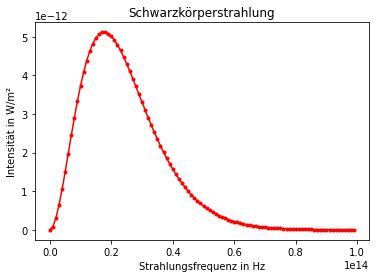
\includegraphics[width=\linewidth]{./gfx/plt-labels}
\end{tcolorbox}
\end{columns}
%
\end{frame}

% =========================================================================== %

\begin{frame}[fragile]
%
\begin{codebox}[Example: Linear and Logarithmic Plot]
\begin{minted}[linenos, fontsize=\scriptsize]{python3}
import matplotlib.pyplot as plt

W  = 500
X  = [x / 10 for x in range(-W, W)]
Y1 = [2 ** x for x in X]
Y2 = [x ** 7 for x in X]

plt.title("Linear Plot")
plt.plot(X, Y1, label="exponential")
plt.plot(X, Y2, label="power")
plt.legend()
plt.show()

plt.title("Logarithmic Plot")
plt.yscale("log")
plt.plot(X, Y1, label="exponential")
plt.plot(X, Y2, label="power")
plt.legend()
plt.show()
\end{minted}
\end{codebox}
%
\end{frame}

% =========================================================================== %

\begin{frame}[fragile]
%
\begin{tcbraster}[raster columns=2,
                  raster equal height,
                  nobeforeafter,
                  raster column skip=0.5cm]
\begin{tcolorbox}[title=Linear Plot]
	\includegraphics[width=\linewidth]{./gfx/plt-linear}
\end{tcolorbox}
%
\begin{tcolorbox}[title=Logarithmic Plot]
	\includegraphics[width=\linewidth]{./gfx/plt-logarithmic}
\end{tcolorbox}
\end{tcbraster}
%
\end{frame}

% =========================================================================== %

\begin{frame}[fragile]{Logarithmic plots}
%
\begin{itemize}
\item Distort one or both axes to show highly dynamic processes
\item Equal distance -- constant factor
\item Commands \texttt{xscale} and \texttt{yscale}
\item Doesn't work for negative values
\item Alternative: \inPy{"symlog"}
	\begin{itemize}
	\item \emph{symmetric logarithmic}
	\item Above [limit] and below -[limit]: logarithmic projection
	\item Between -[limit] and +[limit]: \emph{linear} projection
	\item limit: optional parameters \texttt{linthreshx} or \texttt{linthreshy}, respectively
	\item Set to $\pm 1$ by default
	\end{itemize}
\end{itemize}
%
\end{frame}

% =========================================================================== %

\begin{frame}[fragile]
%
\begin{codebox}[Example: Symmetric Logarithmic Plots]
\begin{minted}[linenos, fontsize=\scriptsize]{python3}
import math
import matplotlib.pyplot as plt

W  = 500
X  = [x / 10 for x in range(-W, W)]
Y1 = [math.sin(x) for x in X]
Y2 = [x / 10      for x in X]

plt.xscale("symlog")
plt.plot(X, Y1)
plt.plot(X, Y2)
plt.grid()
plt.show()

plt.xscale("symlog", linthreshx=10)
plt.plot(X, Y1)
plt.plot(X, Y2)
plt.grid()
plt.show()
\end{minted}
\end{codebox}
%
\end{frame}

% =========================================================================== %

\begin{frame}[fragile]
%
\begin{tcbraster}[raster columns=2,
                  raster equal height,
                  nobeforeafter,
                  raster column skip=0.5cm]
\begin{tcolorbox}[title=symlog{,} default threshold]
	\includegraphics[width=\linewidth]{./gfx/plt-symlog}
\end{tcolorbox}
%
\begin{tcolorbox}[title=symlog{,} explicit threshold]
	\includegraphics[width=\linewidth]{./gfx/plt-symlog-threshold}
\end{tcolorbox}
\end{tcbraster}
%
\end{frame}

% =========================================================================== %

\begin{frame}[fragile]
%
\begin{codebox}[Example: Manually Scaled Axes, width=.53\linewidth, nobeforeafter, equal height group = grpXmpSimplePlotScale]
\begin{minted}[linenos, fontsize=\scriptsize]{python3}
import math
import matplotlib.pyplot as plt

N = 100
X = [(x - N/2) / 10 for x in range(N)]
Y = [math.sin(x) for x in X]

plt.plot(X, Y)
plt.xlim(-6  , +6)
plt.ylim(-0.7, +3)
plt.grid()
plt.show()
\end{minted}
\end{codebox}
%
\begin{tcolorbox}[title=Output: Manually Scaled Axes, width=.45\linewidth, nobeforeafter, equal height group = grpXmpSimplePlotScale]
	\includegraphics[width=\linewidth]{./gfx/plt-limits}
\end{tcolorbox}
%
\end{frame}

% =========================================================================== %

\begin{frame}{More Chart Types!}
%
\begin{itemize}
\item Bar Charts
\item Pie Charts
\item Stacked Plots
\item Scatterplots
\item Histograms
\item Vector Plots
\end{itemize}
%
\end{frame}

% =========================================================================== %

\begin{frame}[fragile]
%
\begin{tcbraster}[raster columns=2,
                  raster equal height,
                  nobeforeafter,
                  raster column skip=0.2cm]
\begin{codebox}[Example: Bar Charts]
\begin{minted}[linenos, fontsize=\scriptsize]{python3}
import matplotlib.pyplot as plt
X = ["Smoot", "Fnord", "R'lyeh"]
Y = [random.randint(0, 11) for x in X]

plt.bar(X, Y, color="#0040B0FF")
plt.ylim(0, 11)
plt.show()

plt.barh(X, Y, color="#0040B0FF")
plt.xlim(0, 11)
plt.show()
\end{minted}
\end{codebox}
%
\begin{tcolorbox}[title=Output: Bar Charts]
	\begin{center}
		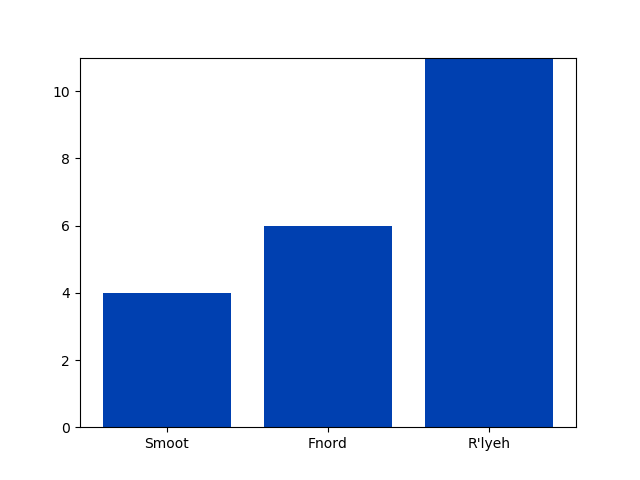
\includegraphics[width=.7\linewidth]{./gfx/plt-bars} \\
		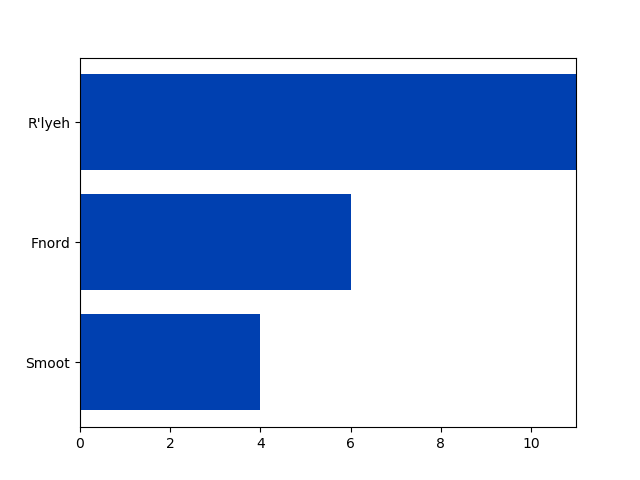
\includegraphics[width=.7\linewidth]{./gfx/plt-barh}
	\end{center}
\end{tcolorbox}
\end{tcbraster}
%
\end{frame}

% =========================================================================== %

\begin{frame}[fragile]
%
\begin{tcbraster}[raster columns=2,
                  raster equal height,
                  nobeforeafter,
                  raster column skip=0.2cm]
\begin{codebox}[Example: Pie Charts (Simple)]
\begin{minted}[linenos, fontsize=\scriptsize]{python3}
import matplotlib.pyplot as plt

contributions = {
    "trial & error"               : 90,
    "searching the web"           : 50,
    "despair, fits of anger, etc" : 10,
    "writing small bits of code"  : 30,
    "brilliant ideas"             : 1
}

plt.pie( contributions.values() )
plt.show()
\end{minted}
\end{codebox}
%
\begin{tcolorbox}[title=Output: Pie Charts (Simple)]
	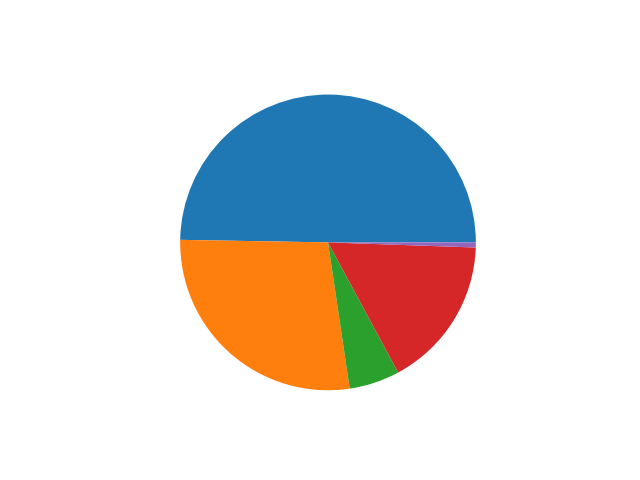
\includegraphics[width=\linewidth]{./gfx/plt-pie-simple}
\end{tcolorbox}
\end{tcbraster}
%
\end{frame}

% =========================================================================== %

\begin{frame}{Pie Charts: Optional Arguments}
%
% itemize[long word] will mess up the left margin, so I hacked that with the weird center/multiline environment
%
\begin{center}
\begin{minipage}{.9\linewidth}
\begin{itemize}
\item[\texttt{labels}] List of strings, labels of the pie slices
\item[\texttt{colors}] List of strings, color names such as \texttt{"red"} or \texttt{"\#FF0000FF"}
\item[\texttt{explode}] List of numbers: how far from center to draw the slice
\item[\texttt{autopct}] String or function. Number Formatting\\
	Strings like \texttt{"5.2f\%"} work like with Format Strings\\
	Functions should take a number between 0 and 100 and compute a string that is used as a label.
\end{itemize}
\end{minipage}
\end{center}
%
\end{frame}

% =========================================================================== %

\begin{frame}[fragile]
%
\begin{codebox}[Example: Pie Charts (Augmented) ...]
\begin{minted}[linenos, fontsize=\scriptsize]{python3}
import matplotlib.pyplot as plt

contributions = {
    "trial & error"                 : 99,
    "searching the web"             : 50,
    "despair, fits of anger, etc"   : 10,
    "writing small bits\n of code"  : 30,
    "brilliant ideas"               : 1
}

def percentToWords(x) :
    if        x <  5 : return "virtually nothing"
    elif  5 < x < 20 : return "a little"
    elif 20 < x < 50 : return "quite a bit"
    else             : return "the majority"
\end{minted}
\end{codebox}
%
\end{frame}

% =========================================================================== %

\begin{frame}[fragile]
%
\begin{codebox}[... continued]
\begin{minted}[linenos, firstnumber=last, fontsize=\scriptsize]{python3}
plt.title("Time Allocation in a coding project")
plt.xlabel("taken from experience")

plt.pie(
    contributions.values(),
    labels=contributions.keys(),
    colors=["#0000AAFF", "blue", "r", "green", "gold"],
    explode=(0, 0.1, 0, 0, .3),
    autopct=percentToWords
)
plt.show()
\end{minted}
\end{codebox}
%
\end{frame}

% =========================================================================== %

\begin{frame}
%
\begin{tcolorbox}[title=Output: Pie Charts (Augmented)]
	\begin{minipage}{.7\linewidth}
	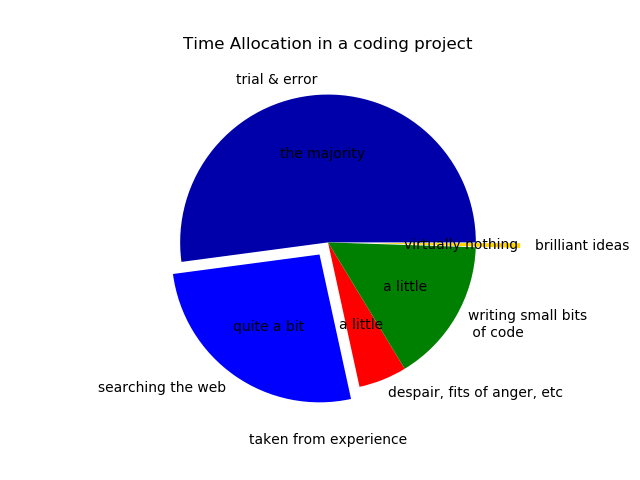
\includegraphics[width=\linewidth]{./gfx/plt-pie-args}
	\end{minipage}
	%
	\begin{minipage}{.25\linewidth}
	\begin{itemize}
	\item Here: Abused the \texttt{xlabel} as a subtitle
	\item \texttt{labels} go outside
	\item \texttt{autopct} texts go inside
	\end{itemize}
	\end{minipage}
\end{tcolorbox}
%
\end{frame}

% =========================================================================== %

\begin{frame}
%
\begin{tcolorbox}[title=Next Goal: Stacked Plots]
\begin{center}
	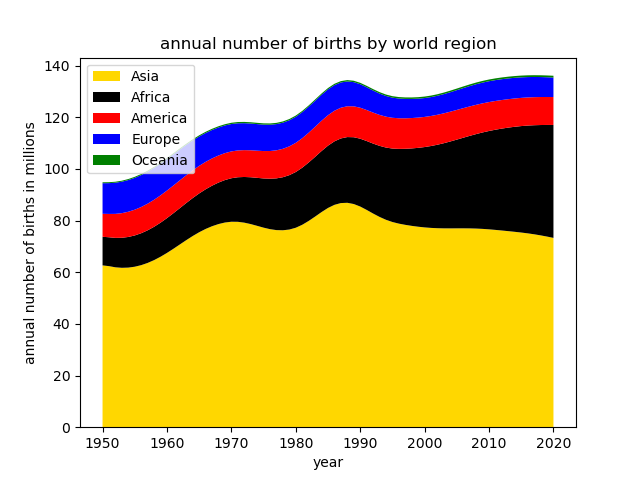
\includegraphics[width=.7\linewidth]{./gfx/plt-stackplot}
\end{center}
\end{tcolorbox}
%
\end{frame}

% =========================================================================== %

\begin{frame}[fragile]
%
\begin{codebox}[Example: Stacked Plots ...]
\begin{minted}[linenos, fontsize=\scriptsize]{python3}
import csv
import matplotlib.pyplot as plt

years    = []
africa   = []
americas = []
asia     = []
europe   = []
oceania  = []
colors   = ["gold", "black", "red", "blue", "green"]

with open("annual-number-of-births-by-world-region.csv", "r") as handle :
    # Data from https://ourworldindata.org/world-population-growth
    # file contains data in this format:
    # Year,Asia,Africa,America,Europe,Oceania
    # 1950,11071.722,8896.969,62638.002,11837.577,360.997
    # 1951,11178.006,9031.823,62344.074,11917.33,366.362
    # ...
      
    reader = csv.reader(handle)
\end{minted}
\end{codebox}
%
\end{frame}

% =========================================================================== %

\begin{frame}[fragile]
%
\begin{codebox}[... continued ...]
\begin{minted}[linenos, firstnumber=last, fontsize=\scriptsize]{python3}
    labels = next(reader)[1:]    # erste Zeile lesen;
                                 # Spaltenüberschriften ohne "Years" übernehmen

    for line in reader :         # verbleibende Zeilen einlesen
        years   .append(float(line[0])       )
        africa  .append(float(line[1]) / 1000)  # line[i] / 1000: file provides
        americas.append(float(line[2]) / 1000)  # birth rate in thousands, but
        asia    .append(float(line[3]) / 1000)  # the plot is better legible
        europe  .append(float(line[4]) / 1000)  # if given in millions.
        oceania .append(float(line[5]) / 1000)


plt.title ("annual number of births by world region")
plt.xlabel("year")
plt.ylabel("annual number of births in millions")
plt.legend(loc="upper left")
\end{minted}
\end{codebox}
%
\end{frame}

% =========================================================================== %

\begin{frame}[fragile]
%
\begin{codebox}[... continued]
\begin{minted}[linenos, firstnumber=last, fontsize=\scriptsize]{python3}
plt.stackplot(
    years,
    asia, africa, americas, europe, oceania,
    labels=labels,
    colors=colors
)

# Alternative way, creates same result:
# data = [asia, africa, americas, europe, oceania]
# plt.stackplot(years, data, labels = labels, colors=colors)

plt.show()
\end{minted}
\end{codebox}
%
\end{frame}

% =========================================================================== %

\begin{frame}{Scatterplots}
%
\begin{itemize}
\item Up to four related quantities in one plot
\item Two coordinates
\item One size information
\item One colour information
\item Example one: Sales strategy for bakery:
	\begin{itemize}
	\item x/y coordinate: fat/sugar content of offered pastries
	\item size: how often customers buy them
	\item colour: bread/sweets/breadrolls/...
	\end{itemize}
\item Example two: Urbanization
	\begin{itemize}
	\item coordinates and population of German cities
	\item colour: status (capital/regular city)
	\end{itemize}
\end{itemize}
%
\end{frame}

% =========================================================================== %

\begin{frame}[fragile]
%
\begin{codebox}[Example: Scatterplots ...]
\begin{minted}[linenos, fontsize=\scriptsize]{python3}
import csv
import matplotlib.pyplot as plt

lat = []      # geographische Länge
lng = []      # geographische Breite
pop = []      # Einwohnerzahl
col = []      # Farbe

colors = {
    "primary" : "red",     # federal capital (Bundeshauptstadt)
    "admin"   : "blue",    # country capital (Landeshauptstadt)
    "minor"   : "black"    # other city
}

# size of dot from population, but small cities should not "vanish"
# ==> cutoff, where dot has minimum size
sizer = lambda x : 0.5 if x < 10000 else x / 10000
\end{minted}
\end{codebox}
%
\end{frame}

% =========================================================================== %

\begin{frame}[fragile]
%
\begin{codebox}[... continued]
\begin{minted}[linenos, firstnumber=last, fontsize=\scriptsize]{python3}
with open("cities-locations-populations-Germany.csv", "r") as handle :
    # Data from https://simplemaps.com/data/de-cities. File Format:
    # city,lat,lng,country,iso2,admin_name,capital,population,population_proper
    # Berlin,52.5167,13.3833,Germany,DE,Berlin,primary,3644826,3644826
    # Hamburg,53.5500,10.0000,Germany,DE,Hamburg,admin,1841179,1841179
    # ...
    reader = csv.reader(handle)
    next(reader)
    for line in reader :
            lat.append(float(line[1]))
            lng.append(float(line[2]))
            pop.append( sizer(float(line[7]))  )
            col.append( colors[line[6]] )

plt.figure(figsize=(6,7.5))
plt.title("Deutschland: Städte")
plt.xlabel("Geographische Länge")
plt.ylabel("Geographische Breite")
plt.scatter(lng, lat, pop, col)
plt.show()
\end{minted}
\end{codebox}
%
\end{frame}

% =========================================================================== %

\begin{frame}
%
\begin{tcolorbox}[title=Next Goal: Stacked Plots]
\begin{center}
	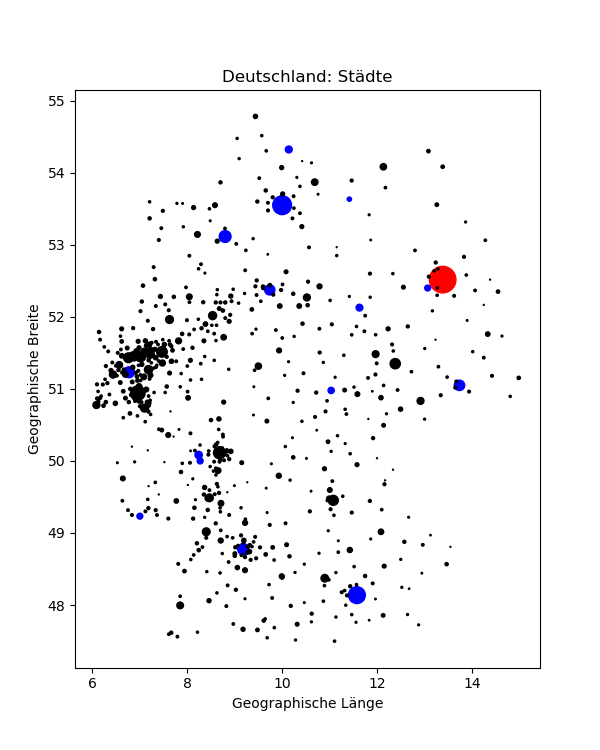
\includegraphics[width=.4\linewidth]{./gfx/plt-de}
\end{center}
\end{tcolorbox}
%
\end{frame}

% =========================================================================== %

\begin{frame}{Histograms}
%
\enquote{Which result occured how many times?}
\begin{itemize}
\item Function \texttt{hist} Automatically classifies data and shows bar plot
\item \texttt{count, bins, patches = plt.hist(data)}
	\begin{itemize}
	\item \texttt{count} is a \inPy{list}, contains how many elements are in class \texttt{i}
	\item \texttt{bins} is a list that contains the lower boundary for each class
	\item \texttt{patches} is an abstract object containing the bars of the plot
	\end{itemize}
\item Number and size of classes can be specified with optional parameters
	\begin{itemize}
	\item \texttt{bins}: \inPy{int}, number of classes to form
	\item \texttt{range}: \inPy{tuple} with the lower and upper boundary of the classes
	\item[\Thus] classes of equal size
	\end{itemize}
\end{itemize}
%
\end{frame}

% =========================================================================== %

\begin{frame}[fragile]
%
\begin{codebox}[Example: Drunk Walk as Histogram ...]
\begin{minted}[linenos, fontsize=\scriptsize]{python3}
import random
import matplotlib.pyplot as plt

runs, N, width, pLeft = 10000, 100, 20, 0.5
drifts = [0] * runs

for run in range(runs) :
    drift  = 0
    for step in range(N) :
        r = random.uniform(0, 1)
        if r < pLeft :
            if drift != -width : drift -= 1
        else :
            if drift != +width : drift += 1
    drifts[run] = drift

plt.title ("Drunk Walk")
plt.xlabel("Drift")
plt.ylabel("Häufigkeit")
\end{minted}
\end{codebox}
%
\end{frame}

% =========================================================================== %

\begin{frame}[fragile]
%
\begin{codebox}[... continued]
\begin{minted}[linenos, firstnumber=last, fontsize=\scriptsize]{python3}
data, bins, patches = plt.hist(drifts, 
                               bins=width+1, range=(-width-1, width+1),
                               histtype='step'
)

print("Histogram Data:")
for b, d in zip(bins, data) :
    print(f"\t{b:+3.0f} through {b+2:+3.0f}: {d:5.0f}")

plt.show()
\end{minted}
\end{codebox}
%
\end{frame}

% =========================================================================== %

\begin{frame}[fragile]
%
\begin{tcbraster}[raster columns=2,
                  raster equal height,
                  nobeforeafter,
                  raster column skip=0.5cm]
\begin{cmdbox}[Terminal: Drunk Walk as Histogram]
\begin{minted}[fontsize=\scriptsize]{text}
Histogram Data:
        -21 through -19:    93
        -19 through -17:   253
        -17 through -15:   254
        -15 through -13:   317
        -13 through -11:   388
        -11 through  -9:   519
         -9 through  -7:   589
         -7 through  -5:   671
         -5 through  -3:   735
         -3 through  -1:   783
         -1 through  +1:   789
         +1 through  +3:   769
         +3 through  +5:   775
         ...
\end{minted}
\end{cmdbox}
%
\begin{tcolorbox}[title=Plot: Drunk Walk as Histogram]
	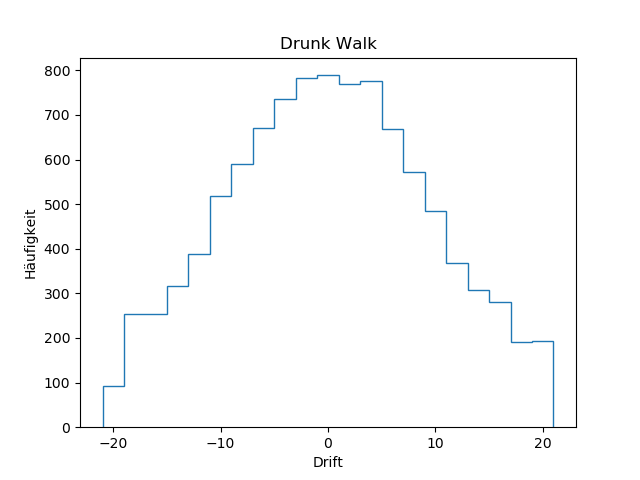
\includegraphics[width=\linewidth]{./gfx/plt-hist-drunkWalk}
\end{tcolorbox}
\end{tcbraster}
%
\end{frame}

% =========================================================================== %

\begin{frame}{Quiver Plots -- Representation of 2D Vector Fields}
%
\begin{itemize}
\item Arrows on a plane
\item Provide four lists
	\begin{itemize}
	\item X- and Y-coordinates where to place the arrows at
	\item x- and y-length of the arrows
	\end{itemize}
\item Or: Provide two lists
	\begin{itemize}
	\item Matrices (lists of lists)
	\item Rows become y-coordinate, columns become x-coordinate
	\item Automatic spacing of 1
	\end{itemize}
\item Or: \enquote{Mixed Form}
	\begin{itemize}
	\item Provide lists of lists and explicit coordinates
	\item MatPlotLib actually ignores inner structure, if four objects are passed
	\item A $2 \times 3$ matrix is equivalent to a list with 6 elements
	\end{itemize}
\end{itemize}
%
\end{frame}

% =========================================================================== %

\begin{frame}[fragile]
%
\begin{codebox}[Example: Quiver Plot]
\begin{minted}[linenos, fontsize=\scriptsize]{python3}
import matplotlib.pyplot as plt

width  = 10
height = 15
xPoints = [x / 10 for x in range(- width, + width)]
yPoints = [y / 10 for y in range(-height, +height)]

X = [xPoints for i in range(2 * height)]   # list of lists!
Y = [[y] * 2 * width for y in yPoints]     # dito!

dataX = []
dataY = []

for y in yPoints :
    for x in xPoints :
        dataX.append(-y)                   # list of numbers
        dataY.append(+x)                   # dito

plt.quiver(X, Y, dataX, dataY)
plt.show()
\end{minted}
\end{codebox}
%
\end{frame}

% =========================================================================== %

\begin{frame}[fragile]
%
\begin{tcolorbox}[title=Quiver Plot]
\begin{center}
	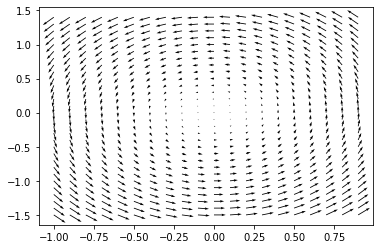
\includegraphics[width=.65\linewidth]{./gfx/plt-vortex}
\end{center}
\end{tcolorbox}
%
\end{frame}

% =========================================================================== %

\begin{frame}{Multiplots}
%
\begin{itemize}
\item Have several plots on one window
\item Command \texttt{plt.subplots(rows, column)}: prepare window
\item Command \texttt{plt.subplot(rows, columns, ID)}: select next drawing spot
	\begin{itemize}
	\item e.\;g. \inPy{plt.subplot(2, 4, 5)}: fifth window of the $2 \times 4$ grid
	\item \ie in row 3, column 1
	\end{itemize}
\item Optional: \inPy{polar = True}
	\begin{itemize}
	\item Use \enquote{x-coordinate} as angle
	\item and \enquote{y-coordinate} as radius
	\end{itemize}
\end{itemize}
%
\end{frame}

% =========================================================================== %

\begin{frame}[fragile]
%
\begin{codebox}[Example: Lissajous-Figures]
\begin{minted}[linenos, fontsize=\scriptsize]{python3}
import math
import matplotlib.pyplot as plt

X = [x / 100 for x in range(628)]
Y = [math.sin(3 * x) for x in X]

plt.subplots(1, 2)
plt.suptitle("Lissajous-Figuren")
plt.subplot(121)
plt.title("Kartesisch")
plt.plot(X, Y)

plt.subplot(122, polar=True)
plt.title("Polarkoordinaten")
plt.plot(X, Y)
plt.show()
\end{minted}
\end{codebox}
%
\end{frame}

% =========================================================================== %

\begin{frame}[fragile]
%
\begin{tcolorbox}[title=Lissajous-Figures]
\begin{center}
	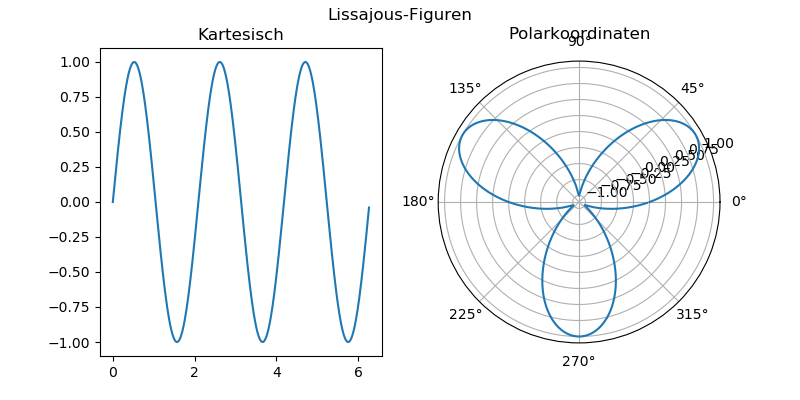
\includegraphics[width=\linewidth]{./gfx/plt-Lissajous}
\end{center}
\end{tcolorbox}
%
\end{frame}

% =========================================================================== %

\begin{frame}{Object Oriented Approach}
%
\begin{itemize}
\item So far: direct commands
\item Actually: act on a class instance maintained by the MatPlotLib
\item We can handle several such objects (several plot windows) manually
\item Slightly different interface, same effects
\item Get a \emph{figure} (\enquote{the plot window}) with \texttt{fig = plt.figure()}
\item Get a \emph{axis object} (\enquote{the subplot region}) with \inPy{drw = fig.add_subplot(rows, columns, ID, projection)}
\item[\Thus] Apply methods to objects
	\begin{itemize}
	\item \inPy{fig.suptitle("some text")} -- headline over all plots
	\item \inPy{drw.set_title("some text")} -- smaller headline for one subplot
	\end{itemize}
\item Axis object often named \texttt{ax}
\end{itemize}
%
\end{frame}

% =========================================================================== %

\begin{frame}[fragile]
%
\begin{codebox}[Example: Lissajous-Figures{,} object oriented approach]
\begin{minted}[linenos, fontsize=\scriptsize]{python3}
import math
import matplotlib.pyplot as plt

X = [x / 100 for x in range(628)]
Y = [math.sin(3 * x) for x in X]

fig = plt.figure(figsize=(8,4))
fig.suptitle("Lissajous-Figuren")

crt = fig.add_subplot(1, 2, 1)
crt.set_title("Kartesisch")
crt.plot(X, Y)

pol = fig.add_subplot(1, 2, 2, projection="polar")
pol.set_title("Polarkoordinaten")
pol.plot(X, Y)
fig.show()

print("Ausgabe noch während der Plot dargestellt wird")
input()
\end{minted}
\end{codebox}
%
\end{frame}

% =========================================================================== %

\begin{frame}{Gridspecs}
%
\begin{itemize}
\item Extended Control over where to place subplots
\item Get a GridSpec object: \texttt{gs = fig.add\_gridspec(rows, columns)}
	\begin{itemize}
	\item Representation of the 2D grid
	\end{itemize}
\item Use the gridspec object to select cells where to place the plot in
	\begin{itemize}
	\item \texttt{fig.add\_subplot(gs[...])}
	\item Indices to subplot: two slices
	\item E.\;g. \texttt{gs[0:2, 1:5]}: $2 \times 4$ block, left uppper is (0, 1)
	\end{itemize}
\end{itemize}
%
\end{frame}

% =========================================================================== %

\begin{frame}[fragile]
%
\begin{codebox}[Example: 2D Normal Distribution ...]
\begin{minted}[linenos, fontsize=\scriptsize]{python3}
import random
import matplotlib.pyplot as plt

N               = 1000
X, Y            = 50, 40
sigmaX, sigmaY  = 5, 10

dataX = [random.gauss(X, sigmaX) for _ in range(N)]
dataY = [random.gauss(Y, sigmaY) for _ in range(N)]

fig = plt.figure(figsize=(8,8))
gs  = fig.add_gridspec(3, 3)

fig.suptitle("2D-Normalverteilung")
fig.subplots_adjust(wspace=0.2, hspace=0.3)

axScatter = fig.add_subplot(gs[0:2, 0:2])
axScatter.set_xlim(0, 100)
axScatter.set_ylim(0, 100)
axScatter.set_xlabel("x")
\end{minted}
\end{codebox}
%
\end{frame}

% =========================================================================== %

\begin{frame}[fragile]
%
\begin{codebox}[... continued]
\begin{minted}[linenos, firstnumber=last, fontsize=\scriptsize]{python3}

axHistX   = fig.add_subplot(gs[ 2 , 0:2], sharex=axScatter)
axHistY   = fig.add_subplot(gs[0:2,  2 ], sharey=axScatter)

axScatter.scatter(dataX, dataY, marker=".")
axHistX.hist(dataX, orientation='vertical'  , bins=20)
axHistY.hist(dataY, orientation='horizontal', bins=20)

fig.show()
input()
\end{minted}
\end{codebox}
%
\begin{itemize}
\item As you see, the number of commands, methods and parameters to memorize piles up quickly
\item Just use your search engine of choice
\item Everything: \url{https://matplotlib.org/stable/api/index.html}
\end{itemize}
%
\end{frame}

% =========================================================================== %

\begin{frame}[fragile]
%
\begin{tcolorbox}[title=2D Normal Distribution]
\begin{center}
	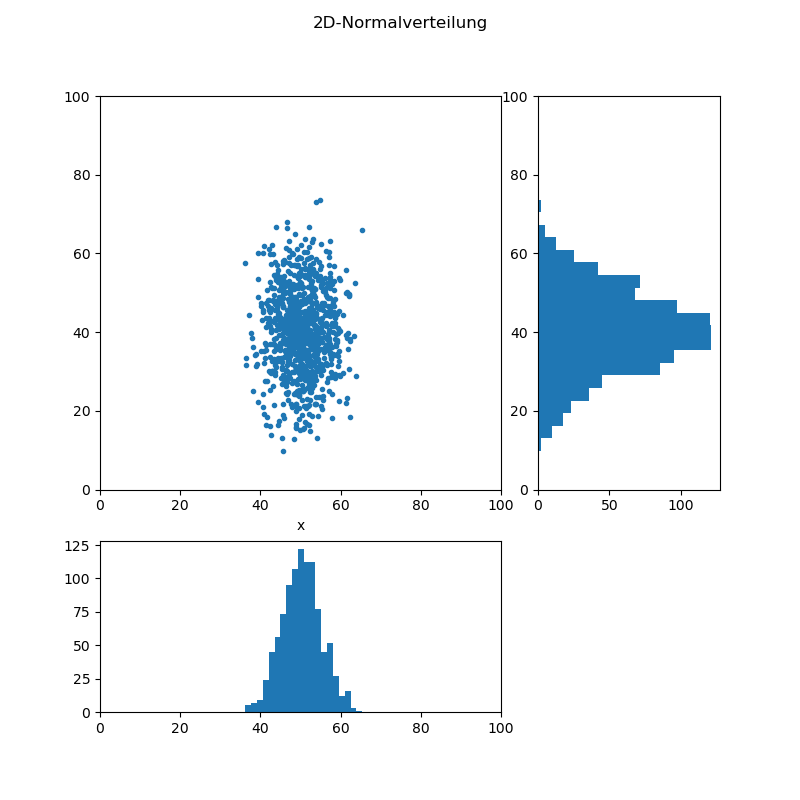
\includegraphics[width=.5\linewidth]{./gfx/plt-gauss2D}
\end{center}
\end{tcolorbox}
%
\end{frame}

% =========================================================================== %

\begin{frame}{Axis Labels}
%
\begin{itemize}
\item \texttt{plt.set\_xticks(where)}, \texttt{plt.set\_yticks(where)}: provide \inPy{list}s of numbers where to put axis labels
\item \texttt{plt.set\_xticklabels(what)}, \texttt{plt.set\_yticklabels(what)}: provide \inPy{list}s of strings what to put there
\item Lists need to be of same length
\item \texttt{set\_*ticklabels}: optional parameter \texttt{fontdict}
\item Formatter: Wrapper to a function that computes text from coordinate value and ID
\item Get via \texttt{formatter = matplotlib.ticker.FuncFormatter(myFunc)}
\item Use via \texttt{drw.yaxis.set\_major\_formatter(formatter)}
\end{itemize}
%
\end{frame}

% =========================================================================== %

\begin{frame}[fragile]
%
\begin{codebox}[Example: Axis Labels]
\begin{minted}[linenos, fontsize=\scriptsize]{python3}
from matplotlib.ticker import FuncFormatter
import matplotlib.pyplot as plt

x = list(range(4))
money = [1.5e5, 2.5e6, 5.5e6, 2.0e7]

fig = plt.figure(figsize=(7,4))
ax = fig.subplots()
ax.bar(x, money)

ax.set_xticks(x)
ax.set_xticklabels( ['Bill', 'Fred', 'Mary', 'Sue'],
                     fontdict={'fontsize' :15, 'fontweight' : 'bold'} )

myTicks = lambda x, pos : f"{(x * 1e-6):1.1f}M, #{pos}"
formatter = FuncFormatter(myTicks)
print(formatter)
ax.yaxis.set_major_formatter(formatter)

plt.show()
\end{minted}
\end{codebox}
%
\end{frame}

% =========================================================================== %

\begin{frame}
%
\begin{tcolorbox}[title=Axis Labels]
\begin{center}
	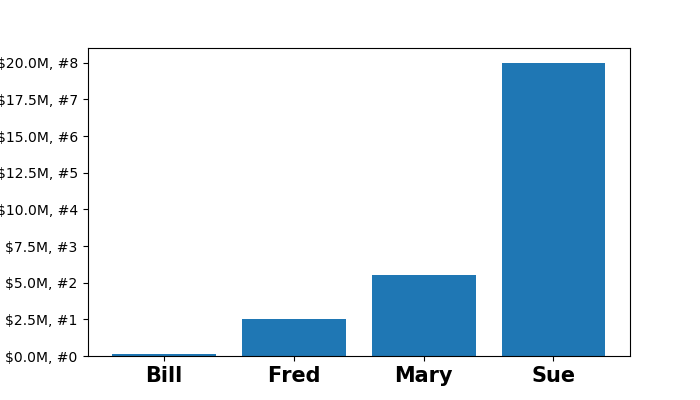
\includegraphics[width=.8\linewidth]{./gfx/plt-TicksFormatter}
\end{center}
\end{tcolorbox}
%
\end{frame}

% =========================================================================== %

\begin{frame}{\LaTeX in Plots}
%
\begin{itemize}
\item Some limited support for \LaTeX
\item Frame String elements in Dollar signs
\item Best: Use raw strings
\item \inPy{r"Normal and $2^{-7}\pi$ LaTex"}
\item Full \LaTeX features: See Script (MatPlotLib can use external \LaTeX compiler)
\end{itemize}
%
\begin{center}
\inPy{plt.title(r"$\frac {\pi }{2} \approx $ 3.1415")}

gives

$\frac{\pi}{2} \approx 3.1415$
\end{center}
%
\end{frame}

% =========================================================================== %

\begin{frame}{Text Overlays}
%
\begin{itemize}
\item Method \texttt{drw.annotate(text, xy=(x, y))}
\item Put \texttt{text} on coordinates \texttt{x, y}
\item Optional parameters \texttt{horizontalalignment} ...
	\begin{itemize}
	\item \inPy{'left', 'center', 'right'}
	\end{itemize}
\item and \texttt{verticalalignment} ...
	\begin{itemize}
	\item \inPy{'top', 'center', 'bottom'}
	\end{itemize}
\item ... and many more ...
\end{itemize}
%
\end{frame}

% =========================================================================== %

\begin{frame}[fragile]
%
\begin{tcbraster}[raster columns=2,
                  raster equal height,
                  nobeforeafter,
                  raster column skip=0.2cm]
\begin{codebox}[Example: Text Overlay]
\begin{minted}[linenos, fontsize=\scriptsize]{python3}
import math
import matplotlib.pyplot as plt

X = [x / 100 for x in range(0, 628, 5)]
Y = [math.sin(t) for t in X]

fig = plt.figure()
drw = fig.subplots()

drw.plot(X, Y)

drw.annotate("Die Sinus-Funktion,\n" +
    "wie von der math-library\n" +
    "zur Verfügung gestellt",
    xy=(3.5, 0.5)
)
plt.show()
\end{minted}
\end{codebox}
%
\begin{tcolorbox}[title=Output: Text Overlay]
	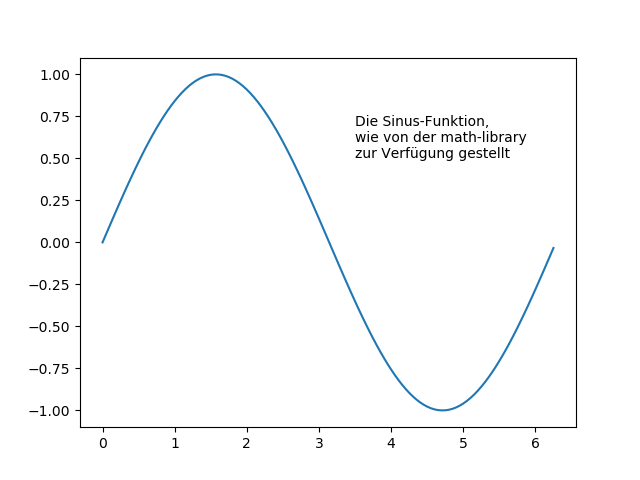
\includegraphics[width=\linewidth]{./gfx/plt-overlay-simple}
\end{tcolorbox}
\end{tcbraster}
%
\end{frame}

% =========================================================================== %

\begin{frame}{Arrows}
%
\begin{itemize}
\item Also with \texttt{drw.annotate}
\item \texttt{textxy} gives foot of arrow (position of text)
\item \texttt{xy} gives head of arrow
\item dict \texttt{arrowprops} gives format specifications
	\begin{itemize}
	\item \texttt{facecolor}
	\item \texttt{edgecolor}
	\item ... and many more
	\item See \url{https://matplotlib.org/stable/api/_as_gen/matplotlib.pyplot.annotate.html}
	\end{itemize}
\end{itemize}
%
\end{frame}

% =========================================================================== %

\begin{frame}{3D Plots}
%
\begin{itemize}
\item Load special submodule:\\
	\inPy{from mpl_toolkits.mplot3d import Axes3D}
\item Use new projection:\\
	\inPy{drw = fig.add_subplot(projection='3d')}
\item Plot now takes three lists \texttt{x, y, z}
\item Commands/Methods \texttt{wireframe} and \texttt{plot\_surface} available (see later)
\end{itemize}
%
\end{frame}

% =========================================================================== %

\begin{frame}[fragile]
%
\begin{codebox}[Example: Axis Labels]
\begin{minted}[linenos, fontsize=\scriptsize]{python3}
import math
import matplotlib.pyplot as plt
from mpl_toolkits.mplot3d import Axes3D

fig = plt.figure()
drw = fig.add_subplot(projection='3d')

T = [math.pi * t / 100 for t in range(1000)]
X = [math.exp(-0.05 * t) * math.cos(t) for t in T]
Y = [math.exp(-0.05 * t) * math.sin(t) for t in T]

drw.set_xlabel("x")
drw.set_ylabel("y")
drw.set_zlabel("time t")
drw.set_title("decaying orbit")
drw.view_init(80, 10)
drw.plot(X, Y, T)
plt.show()
\end{minted}
\end{codebox}
%
\end{frame}

% =========================================================================== %

\begin{frame}
%
\begin{tcolorbox}[title=Axis Labels]
\begin{center}
	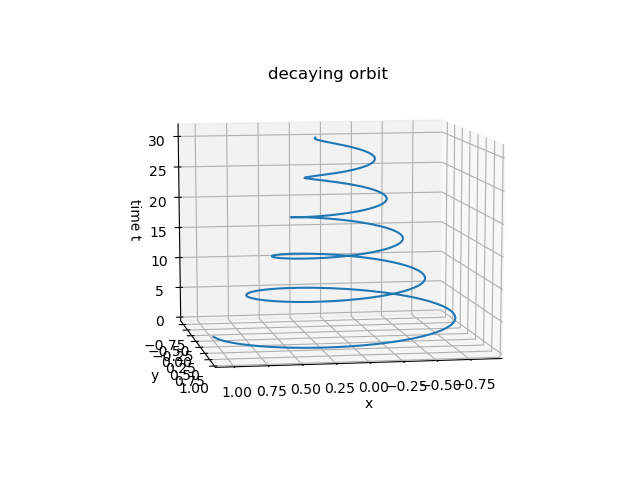
\includegraphics[width=.7\linewidth]{./gfx/plt-orbit3D}
\end{center}
\end{tcolorbox}
%
\end{frame}

% =========================================================================== %

\begin{frame}{Plotting Surfaces}
%
\begin{itemize}
\item Provide three two-dimensional objects: \texttt{X, Y, Z}
\item Same Idea like with the quiver plot
\item \texttt{Z} is height over the baseline
\item Methods actually based on numpy (see tomorrow)
\item[\Thus] Convert to numpy data type
\item 
	\texttt{import numpy as np}\\
	and\\
	\texttt{Z = np.array(Z)}
\end{itemize}
%
\end{frame}

% =========================================================================== %

\begin{frame}[fragile]
%
\begin{codebox}[Example: Data for 3D plots]
\begin{minted}[linenos, fontsize=\scriptsize]{python3}
import numpy as np

W = 20
H = 30

func = lambda x, y : x**2 - y**2

X = [[j/10 - 1.0 for j in range(W)] for i in range(H)]
Y = [[i/10 - 1.5 for j in range(W)] for i in range(H)]
Z = [[None for i in range(W)] for j in range(H)]

for   i in range(H) :
  for j in range(W) :
    x = X[i][j]
    y = Y[i][j]
    Z[i][j] = func(x, y)

Z = np.array(Z)
\end{minted}
\end{codebox}
%
\end{frame}

% =========================================================================== %

\begin{frame}[fragile]
%
\begin{tcbraster}[raster columns=2,
                  raster equal height,
                  nobeforeafter,
                  raster column skip=0.2cm]
\begin{codebox}[Example: Wireframe]
\begin{minted}[linenos, fontsize=\scriptsize]{python3}
import matplotlib.pyplot as plt
from mpl_toolkits.mplot3d import Axes3D

fig = plt.figure()
drw = fig.add_subplot(
    111,
    projection='3d'
)

drw.plot_wireframe(X, Y, Z)

plt.show()
\end{minted}
\end{codebox}
%
\begin{tcolorbox}[title=Output: Wireframe]
	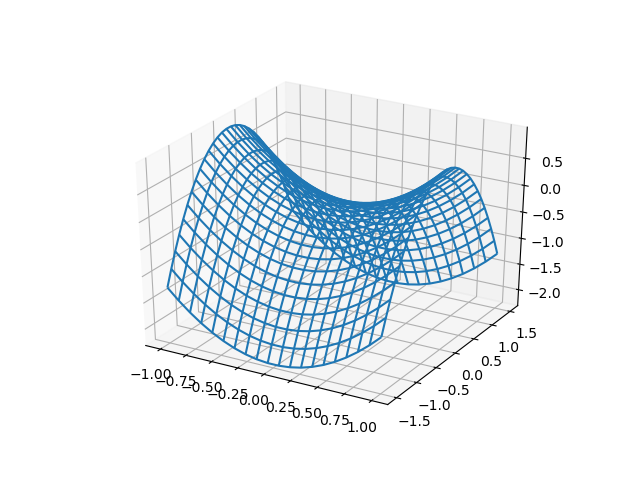
\includegraphics[width=\linewidth]{./gfx/plt-wireframe}
\end{tcolorbox}
\end{tcbraster}
%
\end{frame}

% =========================================================================== %

\begin{frame}[fragile]
%
\begin{tcbraster}[raster columns=2,
                  raster equal height,
                  nobeforeafter,
                  raster column skip=0.2cm]
\begin{codebox}[Example: Wireframe]
\begin{minted}[linenos, fontsize=\scriptsize]{python3}
import matplotlib.pyplot as plt
from mpl_toolkits.mplot3d import Axes3D

fig = plt.figure()
drw = fig.add_subplot(
    111,
    projection='3d'
)

drw.plot_surface(X, Y, Z)

plt.show()
\end{minted}
\end{codebox}
%
\begin{tcolorbox}[title=Output: Wireframe]
	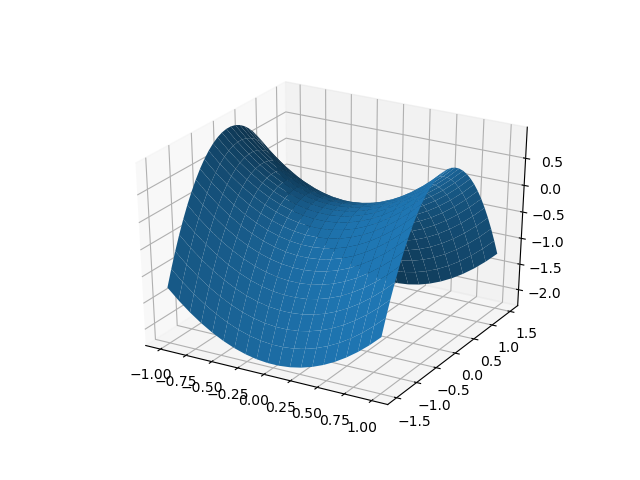
\includegraphics[width=\linewidth]{./gfx/plt-surface3D}
\end{tcolorbox}
\end{tcbraster}
%
\end{frame}

% =========================================================================== %

\begin{frame}[fragile]{Alternative: Heightmaps}
%
\begin{itemize}
\item Use Colour as height information
\item Easier to read
\item No perspective
\item No numpy needed
\item Methods \texttt{pcolor}, \texttt{contour} and \texttt{contourf}
\end{itemize}
%
\begin{codebox}[Example: Heightmaps ...]
\begin{minted}[linenos, fontsize=\scriptsize]{python3}
import matplotlib.pyplot as plt

fig = plt.figure(figsize=(12,4))
grd = fig.add_gridspec(1, 7)
\end{minted}
\end{codebox}
%
\end{frame}

% =========================================================================== %

\begin{frame}[fragile]
%
\begin{codebox}[... continued]
\begin{minted}[linenos, firstnumber=last, fontsize=\scriptsize]{python3}
drw = fig.add_subplot(grd[0,0:2])
drw.set_title("pcolor")
col = drw.pcolor(X, Y, Z)

drw = fig.add_subplot(grd[0,2:4])
drw.set_title("contour")
drw.set_yticks([])
drw.contour(X, Y, Z)

drw = fig.add_subplot(grd[0,4:6])
drw.set_title("contourf")
drw.set_yticks([])
drw.contourf(X, Y, Z)

drw = fig.add_subplot(grd[0,6])
drw.axis("off")
fig.colorbar(col)

plt.show()
\end{minted}
\end{codebox}
%
\end{frame}

% =========================================================================== %

\begin{frame}
%
\begin{tcolorbox}[title=Output: Heightmaps]
	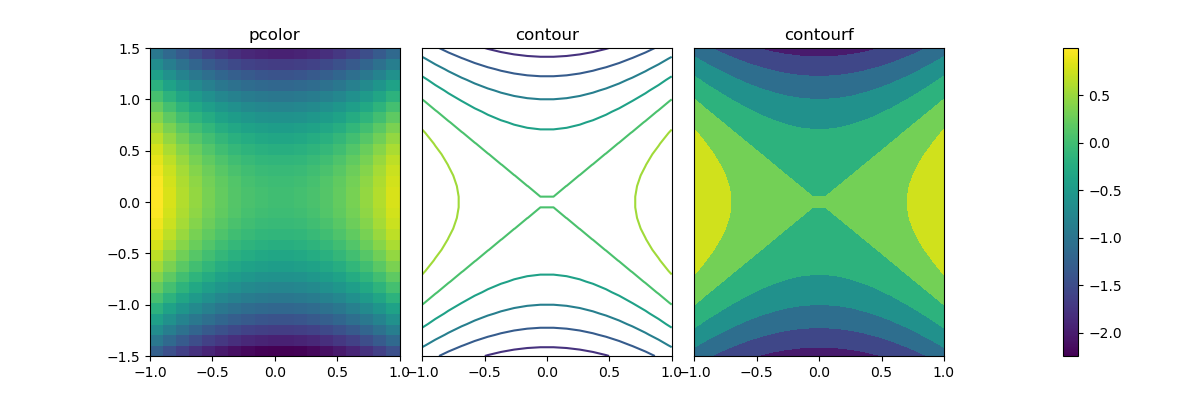
\includegraphics[width=\linewidth]{./gfx/plt-falseColour}
\end{tcolorbox}
%
\end{frame}

% =========================================================================== %

\begin{frame}{Saving Figures to the Hard Disk}
%
\begin{itemize}
\item Method \texttt{fig.safefig}
\item Mandatory parameter filename
\item Extension determines format
\item Supports JPG, PNG, PDF, SVG, ...
\item Optional parameter \texttt{format} fixes file format explicitly
\item See \url{https://matplotlib.org/stable/api/_as_gen/matplotlib.pyplot.savefig.html}
\end{itemize}
%
\end{frame}
\end{document}

% MAREI!!
% whom do I give credit? Where?